%================================================================================
%       Safety Critical Systems Club - Data Safety Initiative Working Group
%================================================================================
%                       DDDD    SSSS  IIIII  W   W   GGGG
%                       D   D  S        I    W   W  G   
%                       D   D   SSS     I    W W W  G  GG
%                       D   D      S    I    WW WW  G   G
%                       DDDD   SSSS   IIIII  W   W   GGG
%================================================================================
%               Data Safety Guidance Document - LaTeX Source File
%================================================================================
%
% Description:
%   Principles and Process section.
%
%================================================================================
\section{Principles and Process (Informative)} \label{bkm:principlesprocess}

\dsiwgSectionQuote{Errors using inadequate data are much less than those using no data at all.}{Charles Babbage}

\subsection{Data Safety Assurance Principles}
Hawkins \dsiwgTextIT{et.\ al.} established some generic software safety assurance principles, which are commonly referred to as ``4 + 1'' \cite{citation:hawkins2013principles}. Given the close links between software and data it is helpful to consider these principles from a data safety assurance perspective. The results are detailed below, with each principle being considered in turn.

\subsubsection{Principle 1: \index{Safety Requirement!Data}Data Safety Requirements shall be defined to address the data contribution to system hazards}
Data pervades active system operation, as well as the system's specification, realisation, verification, validation, certification,  training, maintenance, and retirement. Moreover, data may be passed from one system to another; sometimes over a significant period of time. Data may be assimilated, and converted from prior uses into new uses, or simply used as-is by many systems. It is stored in media whose storage \gls{integrity} decays. The system context for \index{Safety Requirement!Data}Data Safety Requirements may be specific to a particular system's (or [safety] engineering process's) use of the data, or it may be generalised to a class of related systems. Hence \index{Safety Requirement!Data}Data Safety Requirements are needed for any safety-related system that interacts with data.

\subsubsection{Principle 2: The intent of the \index{Safety Requirement!Data}Data Safety Requirements shall be maintained throughout requirements decomposition}
\index{Safety Requirement!Data}Data Safety Requirements establish the system's \index{Property!Safety}safety properties for data, for the system's use of data, for the management of data and for the engineering lifecycle\index{Lifecycle!Engineering} of both the system and its associated data. The system's requirements hierarchy must preserve the intent of the \index{Safety Requirement!Data}Data Safety Requirements (and hence the system's safety-related \index{Property!Data}\glspl{data property}). Moreover, the applied engineering process for both the system's realisation and subsequent lifecycle\index{Lifecycle!System} stages shall demonstrate that the data safety properties are preserved.

\subsubsection{Principle 3: \index{Safety Requirement!Data}Data Safety Requirements shall be satisfied}
Evidence is required that the system satisfies all of the \index{Safety Requirement!Data}Data Safety Requirements imposed on it for all anticipated operating conditions. Moreover, the \index{Safety Requirement!Data}Data Safety Requirements that pertain to the data's lifecycle\index{Lifecycle!Data} outside of the system shall be evidentially demonstrated prior to the system acting on such data, or else the system shall be able to adequately defend against unsatisfied \index{Safety Requirement!Data}Data Safety Requirements. In other words, either the data can be shown to demonstrate the required \index{Property!Data}\glspl{data property} prior to being used, or the system can implement adequate defences and mitigations\index{Mitigation} against data that does not conform to the required \index{Property!Safety}safety properties.

\subsubsection{Principle 4: Hazardous system behaviour arising from the system's use of data shall be identified and mitigated\index{Mitigation}}
This is an intentionally broad statement because data is conceptual and not physical; it is the contextualised use of data that could result in a system hazard. Data Safety Assurance Principle 1 deals with system-level hazards arising from data, whereas Data Safety Assurance Principle 4 is concerned with hazards that arise from the way the system uses its data; that is, whether the system's design and implementation introduce further hazards. An example is a ship navigation system's display of hydrographic chart data, where a wide field display results in small features disappearing (due to image scale) when it is critical that situational awareness of such hazards is maintained.

\subsubsection{Principle 4+1: The confidence established in addressing the Data Safety Assurance Principles shall be commensurate to the contribution of the data to system risk}
The confidence in the evidence that demonstrates establishment of the first four Data Safety Assurance Principles shall be proportionate to the contribution data (or a particular \index{Artefact, Data}\gls{data artefact}) makes to the system hazards.

\subsection{Data Safety Management Process}
To assist organizations with integrating data safety considerations into their existing processes and,
in due course, their Safety Management System, an outline Data Safety Management Process has
been developed.

This is structured around ISO 31000 \cite{citation:iso310002018risk}, and takes into account the Data Safety Assurance Principles:
links between the process objectives and the assurance principles are described in \autoref{bkm:principlesobjectives}. The
adoption of ISO 31000 means that a relatively simple process, which focuses on data-related
aspects, can be presented here and applied by individual organizations.

To simplify the presentation, the process is presented as a series of sequential phases. In practice, a
degree of iteration is likely to be required (e.g., measures adopted to treat risks may lead to refined
system design and revised risk analyses). Likewise, it may be appropriate for some parts of the
process to run in parallel (i.e., a subsequent phase may start before a preceding phase has finished).
\begin{figure}[h]
\centering
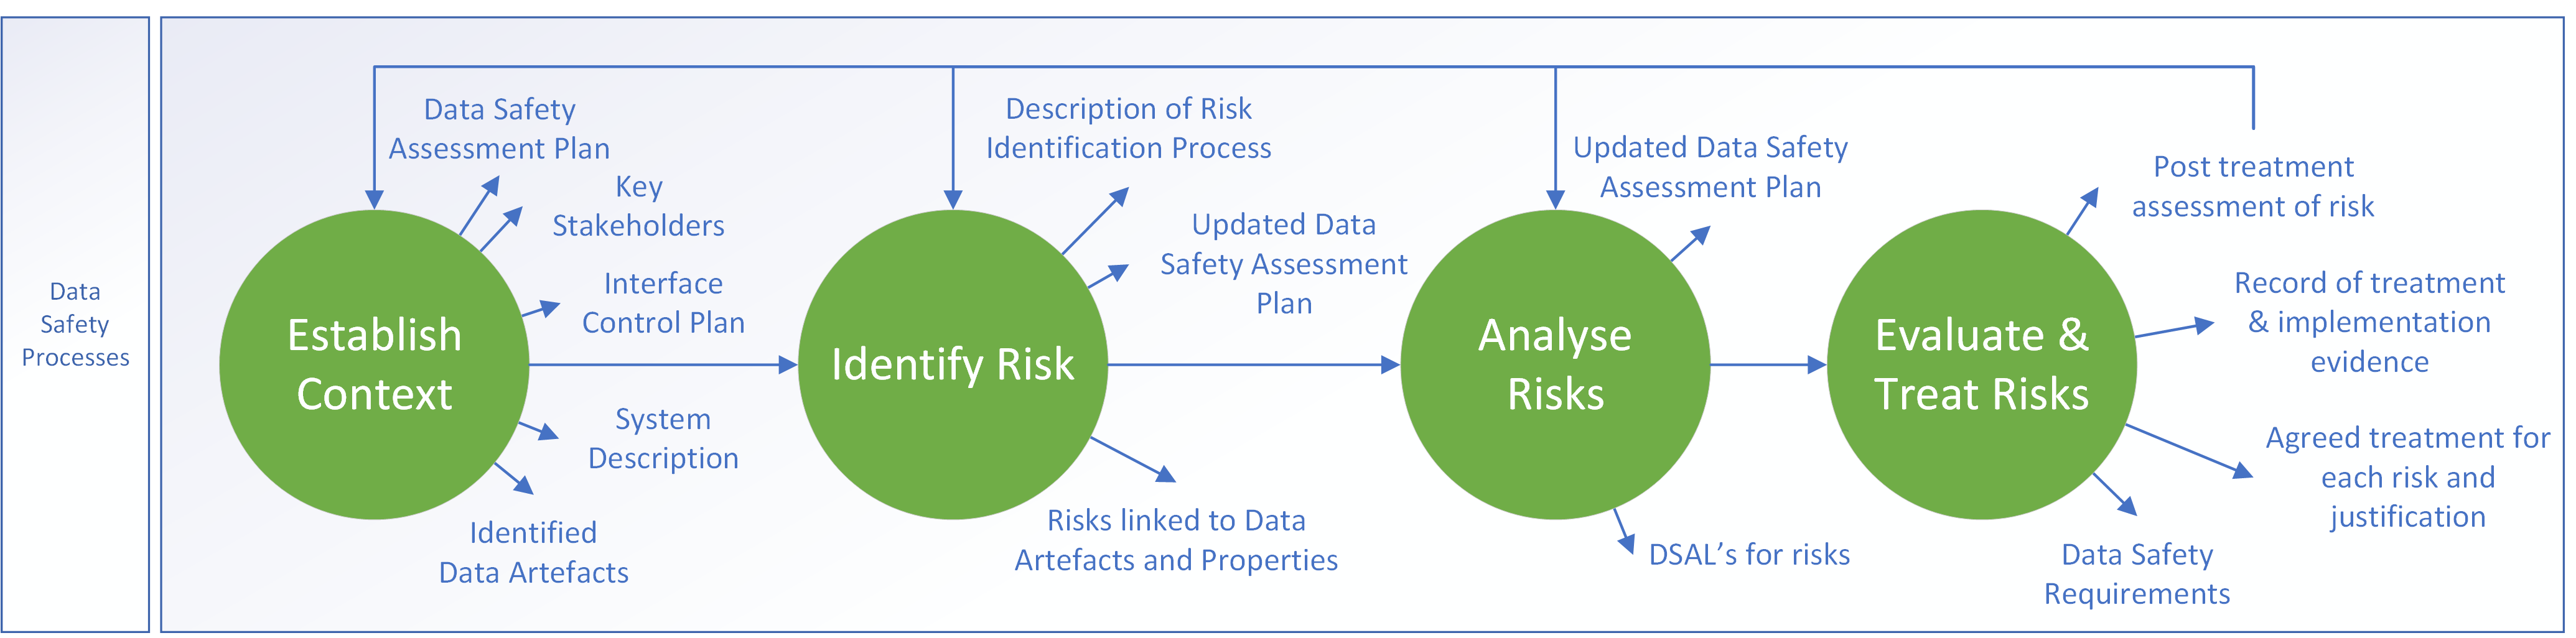
\includegraphics[scale=0.45]{images/process diagram v3 Data Safety Only}
\caption{Process Phases}
\label{fig:process_phases}
\end{figure}

The Data Safety Management Process occurs over four key steps as shown in \autoref{fig:process_phases}, and the specific
objectives and outputs of each step are described in more detail in \autoref{bkm:objectivesoutputs}. The last outcome of the
process is a `Post treatment risk assessment'. If the risk reduction is not considered adequate then
the process will iterate again. The whole process is intended to be repeated through the lifecycle of
the system and so will be repeated many times and further iterations will be required when there
are changes to the system or its data.

Although the Data Safety Management Process is based on the structure of ISO 31000, there are
some differences between the two. These include:
\begin{itemize}
\item The ISO standard’s ``Establish Context'' phase is concerned with an organization adopting a
	risk management system; within this guidance document that phase is extended to apply to
	specific projects;
\item The ISO standard considers risk as being synonymous with uncertainty in outcome (i.e.,
	some risks may be beneficial and hence it may be desirable to take actions to increase their
	likelihood); within this guidance document all risks are considered to have adverse effects;
	and
\item The ISO standard separates the ``Evaluate Risks'' and ``Treat Risks'' activities; within this
	guidance document it has been convenient to combine these into a single phase.
\end{itemize}

ISO 31000 also recommends two activities that run in parallel with risk assessment. These activities
are:
\begin{enumerate}
\item monitor and review the risk assessment process; and 
\item communicate and consult with the
Stakeholders about the risk assessment process. 
\end{enumerate}
Aspects like ``monitor'', ``review'', ``communicate''
and ``consult'' are taken to be part of normal project activities; items like the \gls{odr} assessment and
the \gls{dsmp} are intended to assist from the perspective of data safety.

\subsection{Data Safety Management Process Overview}
\begin{figure}[hb]
\centering
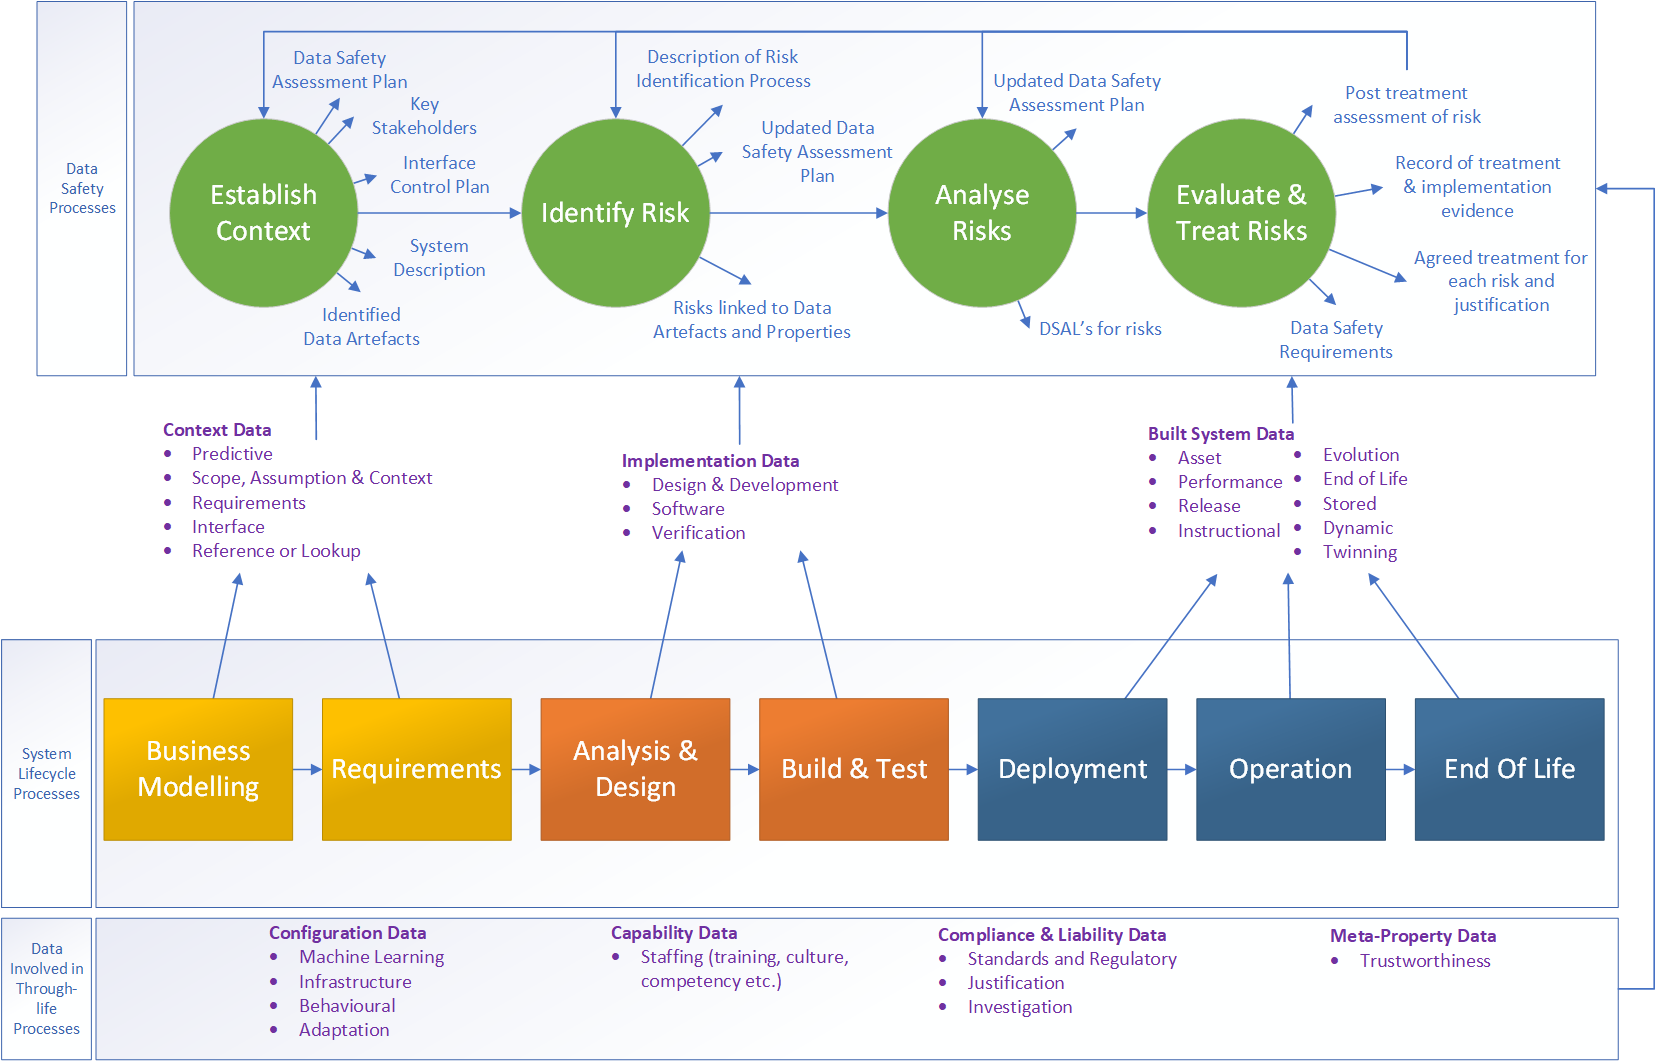
\includegraphics[angle=90,scale=0.7]{images/process_diagram}
\caption{Simplified Process Overview}
\label{fig:process}
\end{figure}

\autoref{fig:process} provides an overview of how the of the \gls{dsmp}
integrates with a typical system lifecycle. In practice, the main \cbstart\gls{safety assessment}\cbend\ activities will
occur as part of the normal safety assessment process lifecycles, so for example, when risks arising
from failures of the software and hardware of a system, loss of properties of data should also be
considered. However, data pervades all aspects of a systems lifecycle so the \gls{safety assessment}
process can occur throughout the system lifecycle depending on the type of data that is being
assessed. Some \glspl{item data} such as Context, Implementation and Built System Data are relevant for
specific process phases of the lifecycle, while others such as Configuration, Capability, Compliance and
Liability Data apply throughout the entire lifecycle. The Meta-Property Data of Trustworthiness
covers data that is used to inform on the overall trustworthiness of the system. The specific data
categories are covered in more detail in \autoref{bkm:datacategories}.

The bottom section of the figure shows a typical basic lifecycle for a system from its inception
through to end of life. The types of data that are of concern for each process step including those
that apply to all steps are shown and these feed into the data \gls{safety assessment} process. Further
examples of lifecycles are given in \autoref{bkm:lifecycle}.
\cbend

%\newpage
%\subsection{Summary Figure}
%\begin{figure}[!h]
  %\centering
  %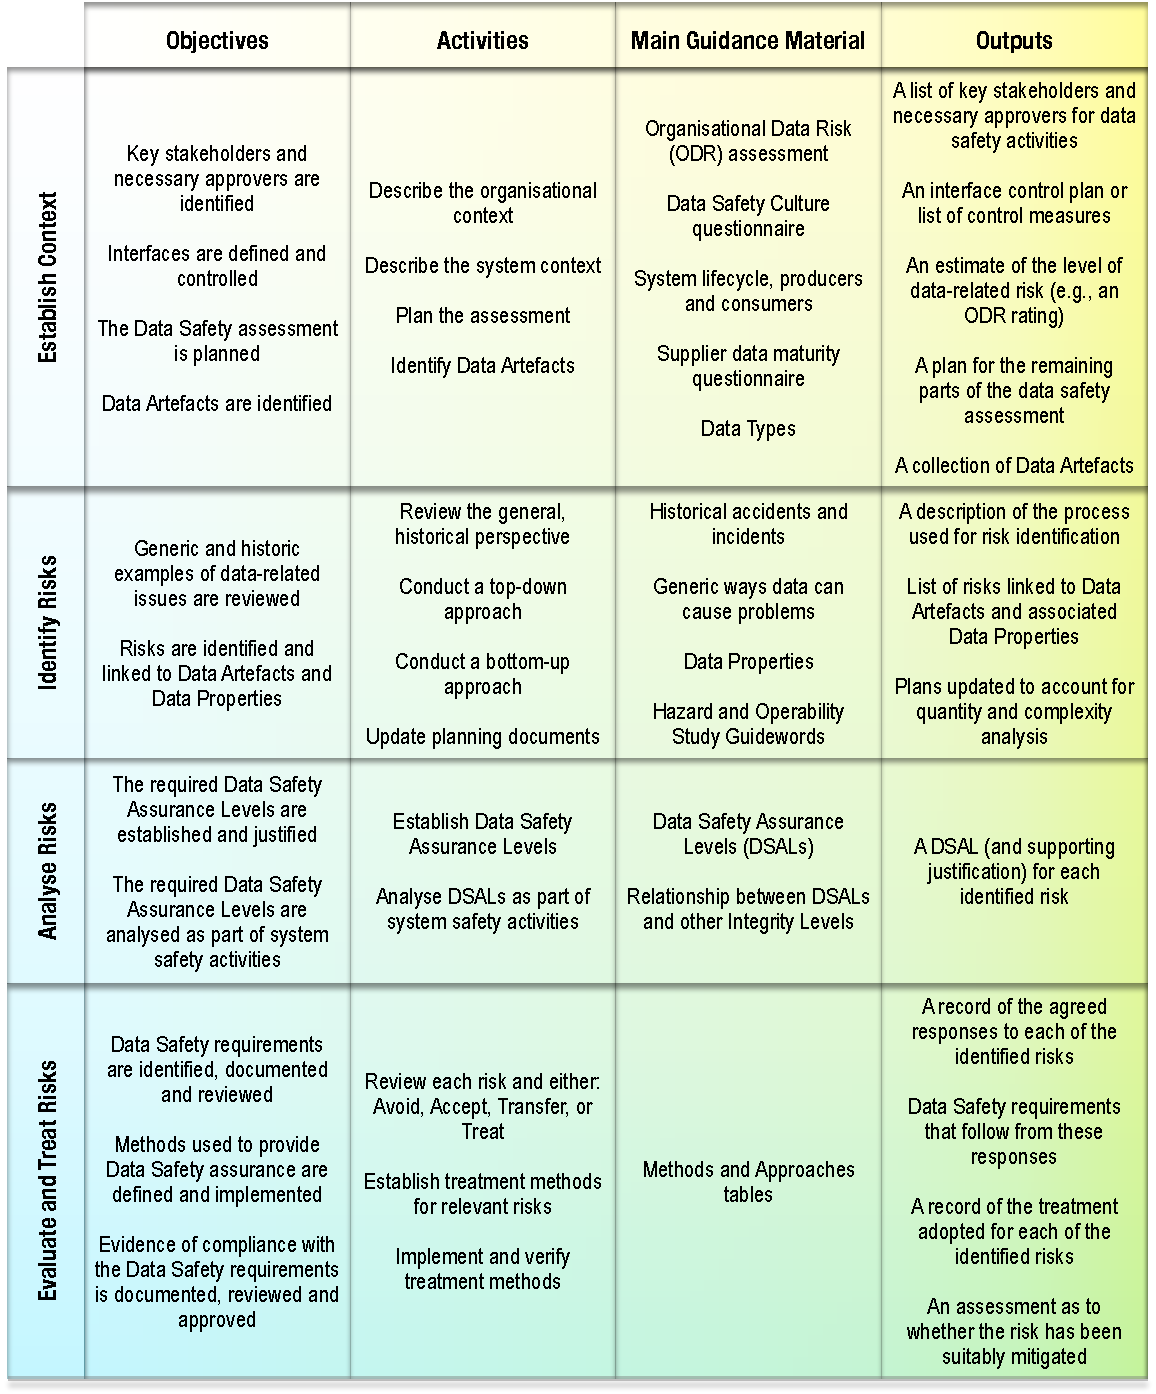
\includegraphics[width=\textwidth]{images/summaryfigure}
  %\label{fig:summaryfigure}
%\end{figure}
